\chapter{Kanalcodierung}
\begin{center}
	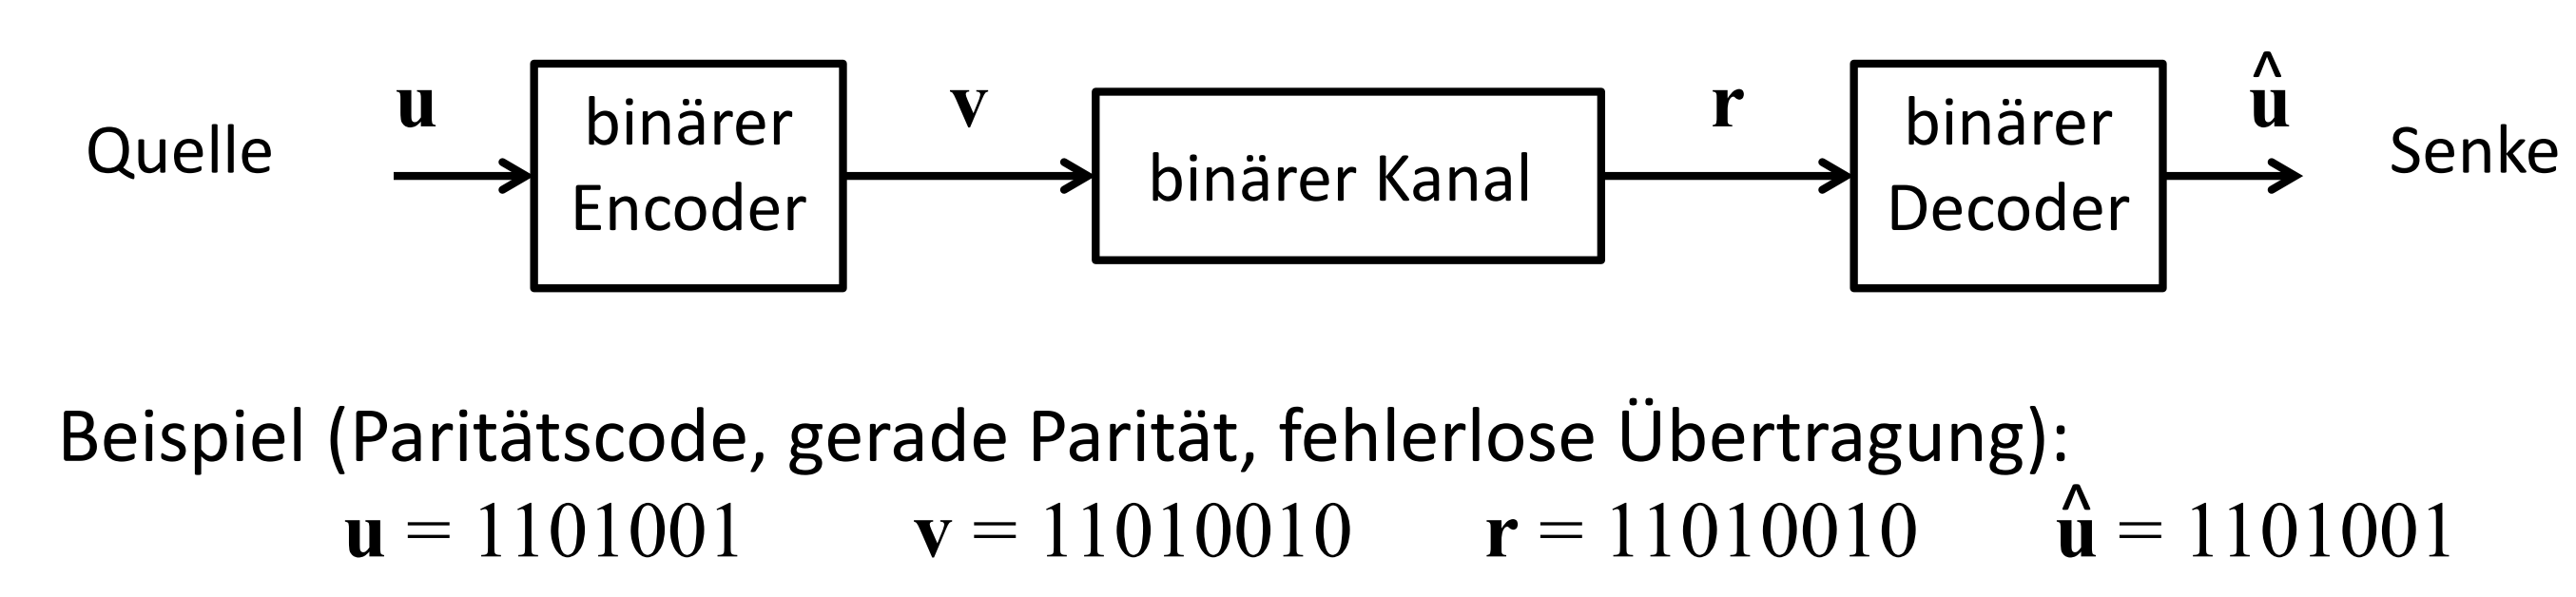
\includegraphics[width=.9\textwidth]{./images/bincode.png}
\end{center}
\section{Paritätscode}
Nachricht:
\[ \textbf{u} = \underbrace{
	\begin{bmatrix}1 & 1 & 0 & 1 & 0 & 0 & 1\end{bmatrix}
	}_\textrm{$k$ bits} \]
~\\
Codewort:
\[ \textbf{v} = \underbrace{
	\begin{bmatrix}1 & 1 & 0 & 1 & 0 & 0 & 1 & 0\end{bmatrix}
	}_\textrm{$n$ bits} \]
~\\
Coderate:
\[ R = \frac{k}{n} \]
\section{Repetitionscode}
Jedes Bit wird $N$-mal wiederholt, somit ist die Coderate $\frac{1}{N}$.

\section{Generatormatrix}
Nachricht \textbf{u}: Zeilenvektor der Länge $k$\\
Codewort \textbf{v}: Zeilenvektor der Länge $n$\\
Generatormatrix \textbf{G}: ($k\times n$)-Matrix\\
\[ \textbf{v} = \textbf{u} \cdot \textbf{G} \]
~\\
Hamming Code (7,4):
\[ G_{n=7,k=4} = \begin{bmatrix}
	1 & 0 & 0 & 0 & 1 & 0 & 1 \\
	0 & 1 & 0 & 0 & 1 & 1 & 0 \\
	0 & 0 & 1 & 0 & 1 & 1 & 1 \\
	0 & 0 & 0 & 1 & 0 & 1 & 1 \\
\end{bmatrix} \]
~\\
\textbf{Linearität}: Zur Berechnung z.B. der minimalen Hamming-Distanz des Codes darf wegen 
der Linearität stets das Codewort  \textbf{v = 0} als Referenz genommen werden.
\\\\
Aufbau:
\[ \textbf{G} = \left[\textbf{I}_k|\textbf{P}_{k\times (n-k)}\right] \]
~\\
Party-check Matrix:
\[ \textbf{H} = \left[\textbf{P}^T | \textbf{I}_{n-k}\right] \]
~\\
Empfangener Symbolvektor:
\[ \textbf{r} = \textbf{u} \cdot \textbf{G} + \textbf{n} \]
~\\
Syndrom:
\[ \textbf{s} = \textbf{r} \cdot \textbf{H}^T = \textbf{n} \cdot \textbf{H}^T \]

\section{Optimale Decodierung}
AWGN Kanal mit bin. Eingang:
\[ p(r_i|V_i=1) = \frac{1}{\sqrt{2\pi\sigma^2}} \e^{-\frac{(r_i-1)^2}{2\sigma^2}} \]
\[ p(r_i|V_i=0) = \frac{1}{\sqrt{2\pi\sigma^2}} \e^{-\frac{(r_i+1)^2}{2\sigma^2}} \]

\begin{center}
	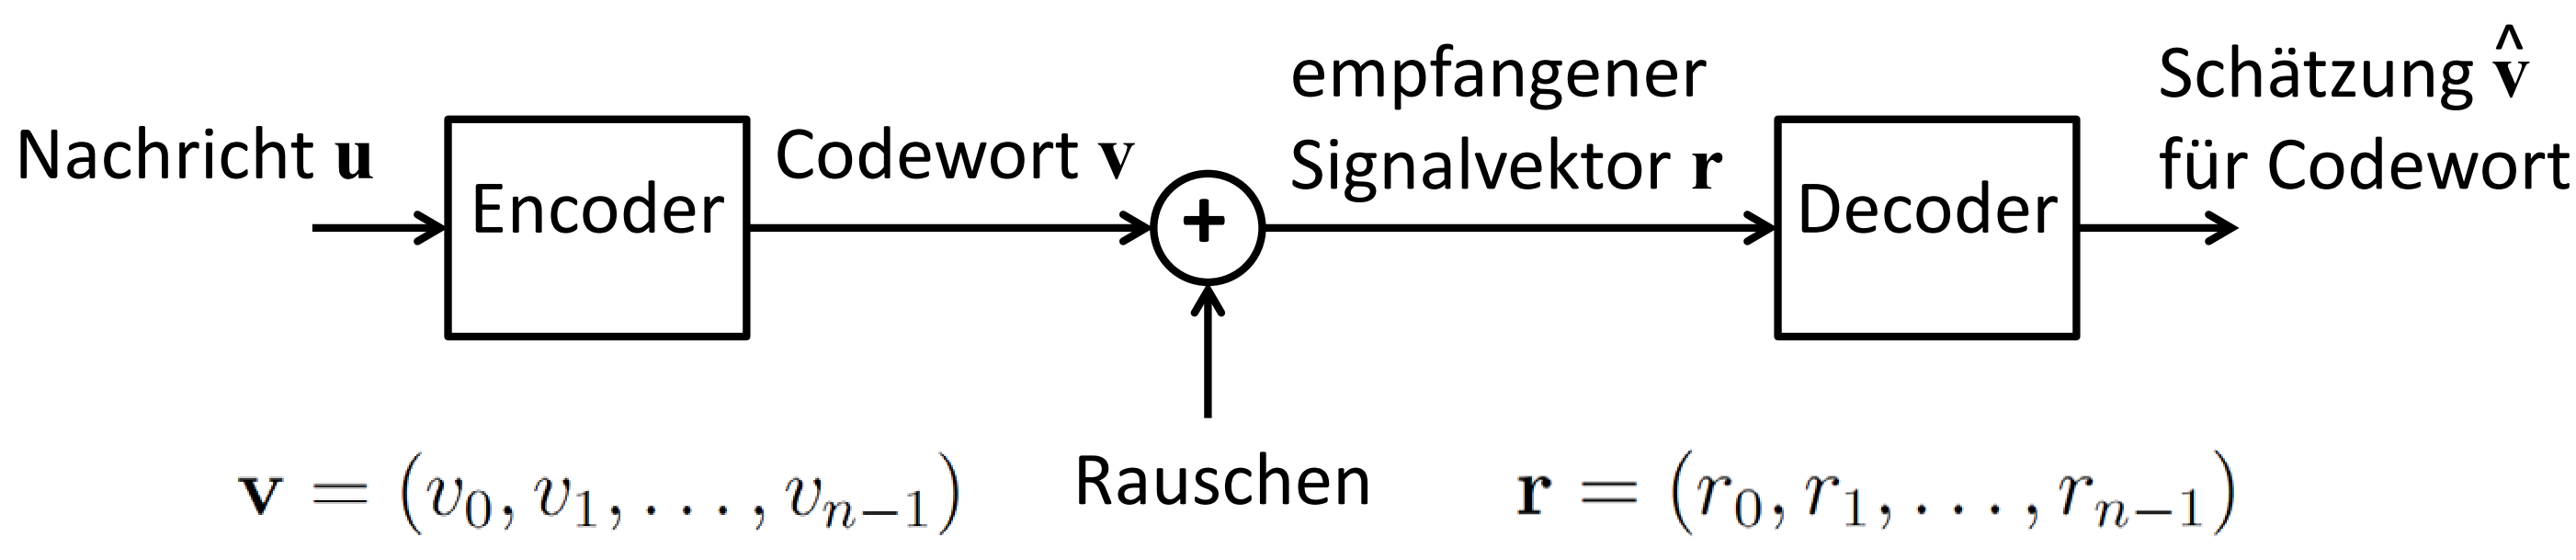
\includegraphics[width=.9\textwidth]{./images/optdecode.png}
\end{center}
Satz von Bayes:
\[ p(y_j|x_i) = \frac{p(y_j) \cdot p(x_i|y_j)}{p(x_i)} \]
Maximum a posteriori Schätung:
\[ \hat{\textbf{v}} = \arg\max p(\textbf{v}|\textbf{r}) \]
~\\
Maximum-Likelihood Decodierung:
\[ \hat{\textbf{v}} = \arg\max p(\textbf{r}|\textbf{v}) =
	\arg\max\log p(\textbf{r}|\textbf{v}) \]
~\\
Log-likelihood-Funktion:
\[ \log p(\textbf{r}|\textbf{v}) = \sum_{i=0}^{n-1} \log p(r_i|v_i) \]
~\\
Liklihood-Verhältnis:
\[ \frac{p(r_i|V_i=1)}{r_i|V_i=0} \]
~\\
Log-Liklihood ratio:
\[ \Lambda(r_i) = \log\frac{p(r_i|V_i=1)}{r_i|V_i=0} \]
\[ \Lambda(r_i) = \frac{2r_i}{\sigma^2} \qquad \textrm{für bin AWGN Kanal}\]
~\\
Branch-Metrik:
\[ L_i(v_i) = \left\lbrace \begin{matrix}
		\Lambda(r_i)  & \textrm{für } v_i=1\\
		-\Lambda(r_i) & \textrm{für } v_i=0\\
	\end{matrix} \right. \]
~\\
Pfadmetrik:
\[ L(\textbf{v}) = \sum_{i=0}^{n-1}L_i(v_i) \]

\section{Faltungscodes}
($n,k,m$)-Faltungscode:
\begin{itemize}
	\item $n$: Anzahl Ausgangsbits pro Takt
	\item $k$: Anzahl Eingangsbits pro Takt
	\item $m$: Anzahl innere Speicher
\end{itemize}
~\\
Rate: $\frac{k}{n}$

\begin{center}
	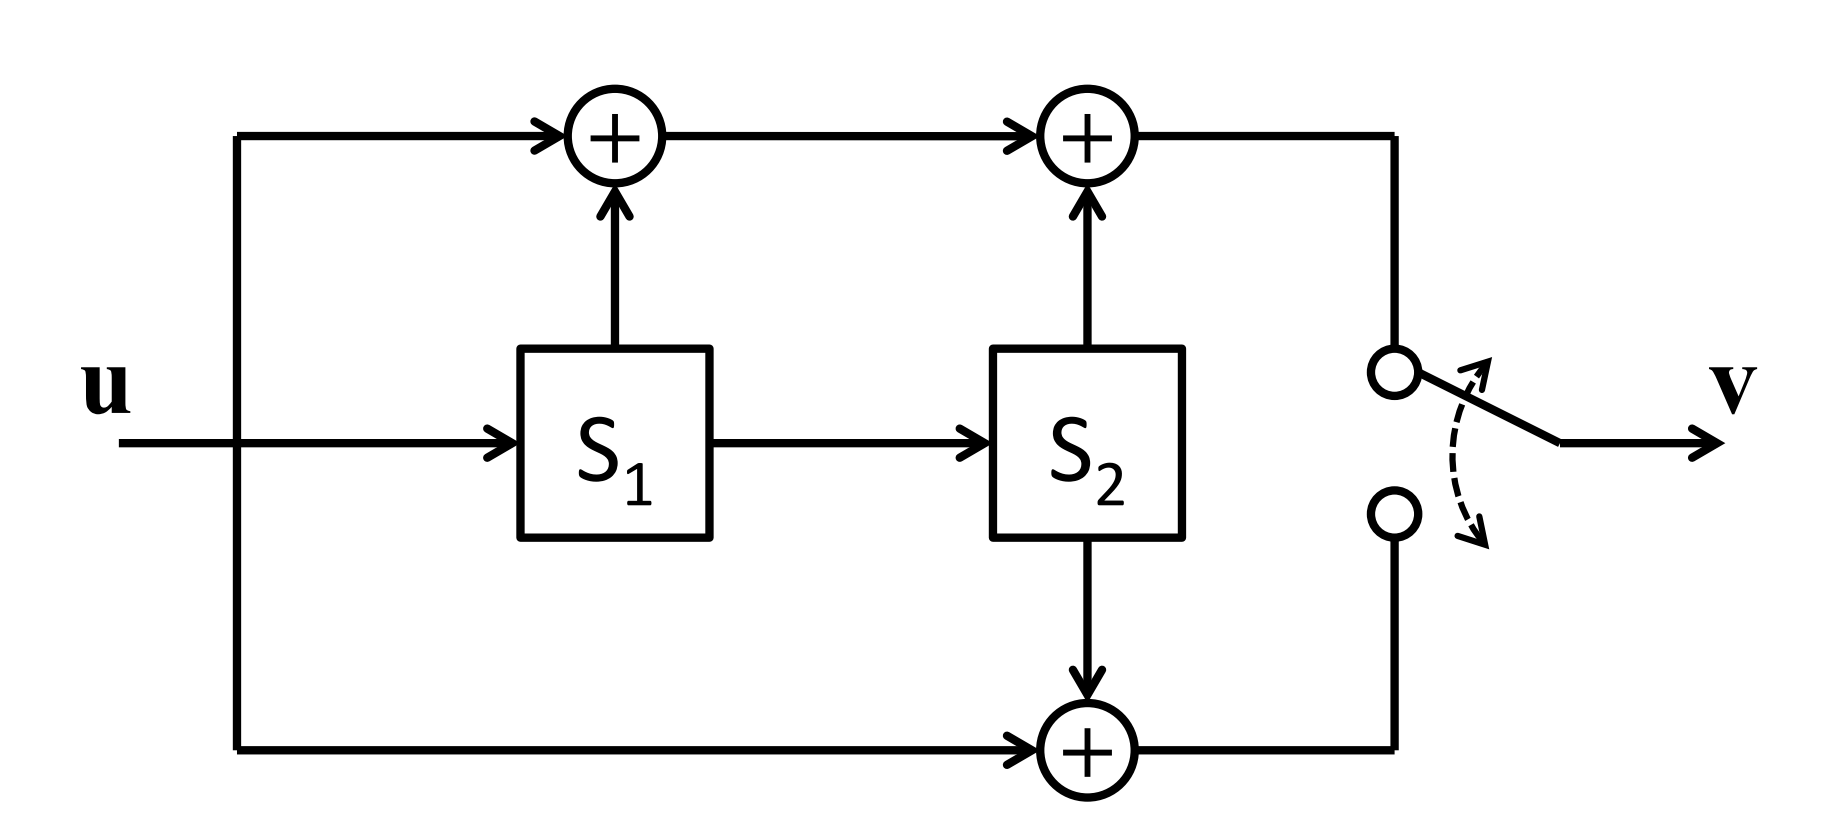
\includegraphics[width=.9\textwidth]{./images/faltungscode.png}
\end{center}

\begin{center}
	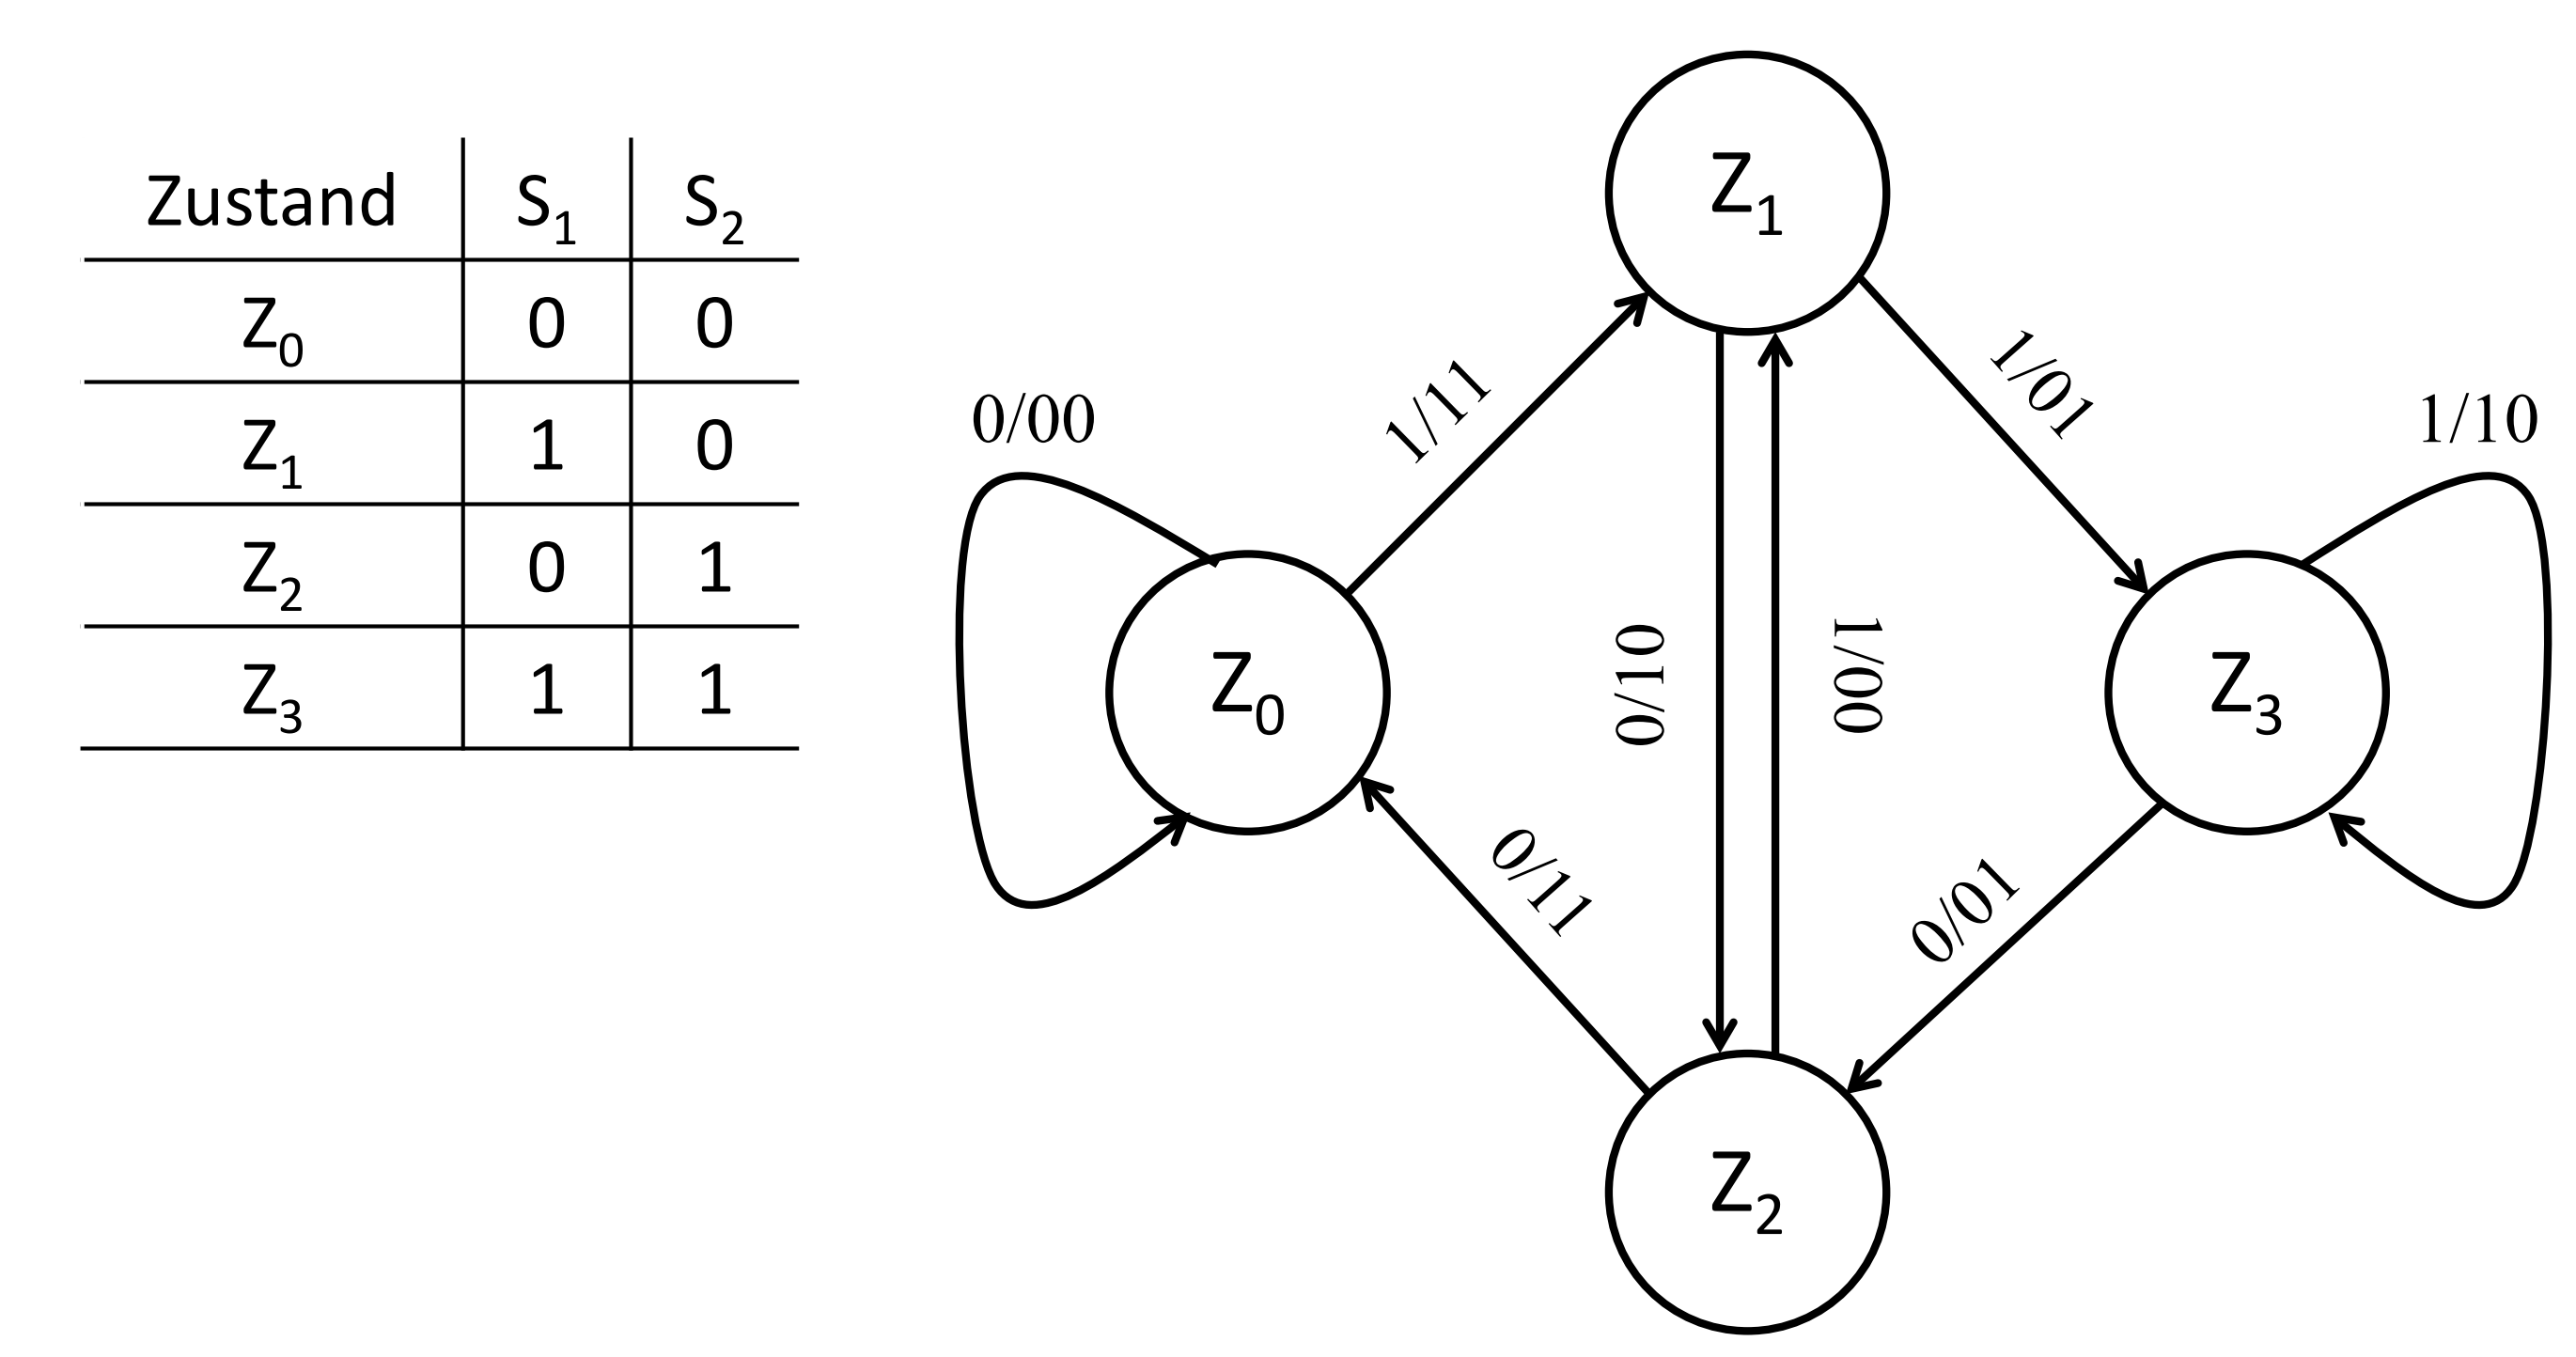
\includegraphics[width=.9\textwidth]{./images/zustand.png}
\end{center}